\documentclass[a4paper]{article}

%% Language and font encodings
\usepackage[ngerman]{babel}
\usepackage[utf8x]{inputenc}
\usepackage[T1]{fontenc}

%% Sets page size and margins
\usepackage[a4paper,top=3cm,bottom=2cm,left=3cm,right=3cm,marginparwidth=1.75cm]{geometry}
%\usepackage{a4wide}
\usepackage[onehalfspacing]{setspace}

%% Useful packages
\usepackage{amsmath}
\usepackage{graphicx}
\usepackage[colorinlistoftodos]{todonotes}
\usepackage[colorlinks=true, allcolors=blue]{hyperref}
\usepackage{csquotes}
\usepackage{listings}
\usepackage{siunitx}

\title{SenPi - Smart Environment}
\author{Adrian Herrmann, Niclas Kristek, Iman Nouri-Namini, Thomas Tegethoff}

\begin{document}
\maketitle

\section{Einführung}

Das Ziel des SenPi Smart-Environment-Projekts ist die Sammlung und Visualisierung verschiedener Sensordaten. Zu diesem Zweck wird ein Board mit integrierten oder extern angeschlossenen Sensoren mit einer RIOT-basierten Applikation bestückt, das die Daten der angeschlossenen Sensoren sammelt und an ein Raspberry Pi verschickt, welches die Daten in einer Datenbank speichert, die einem Webserver zur Verfügung steht. Zusätzlich können Sensordaten über an das Board angeschlossene LED-Streifen visualisiert werden. Es wird ein Phytec phyNODE KW22 benutzt, aber die Anwendung ist so geschrieben, dass beliebige Boards benutzt werden können, auf denen RIOT läuft. In diesem Bericht wird der Aufbau des Projekts beschrieben und Entscheidungen zur Architektur erläutert sowie auf Fehlschläge und noch anstehende Herausforderungen eingegangen.

\section{SenPhy}
Die SenPhy-Anwendung ist RIOT-basiert. Die Wahl von RIOT als IoT-Betriebssystem war naheliegend, da RIOT von vielen FU-Mitarbeitern mitentwickelt wird (inklusive der Betreuer des Softwareprojekts) und somit direkte Unterstützung vorhanden war. SenPhy liest die Werte der angeschlossenen Sensoren aus und überträgt sie auf Anfrage an den Server. Auch wenn die Anwendung theoretisch auf allen Boards, die von RIOT unterstützt werden, laufen sollte, wird primär das Phytec-phyNODE-KW22 verwendet, weil es bereits über eine Vielzahl vormontierter Sensoren verfügt. Bei diesen Sensoren handelt es sich um:
\begin{enumerate}
	\item Thermometer
    \item Luftfeuchtigkeitssensor
    \item RGB-Lichtsensor
    \item Magnetometer
    \item Gyroskop
    \item Drucksensor
    \item kapazitiver Taster
\end{enumerate}
Lediglich die Werte des kapazitiven Tasters werden nicht für Abfragen zur Verfügung gestellt, da es für ihn keinen Treiber gibt, der die SAUL-API implementiert und weil er streng genommen keine Umweltwerte darstellt. Die SAUL-API stellt eine einheitliche Schnittstelle für Gerätetreiber in RIOT dar und ermöglicht somit eine einfache Austauschbarkeit und Erweiterbarkeit von Sensoren.

Bei der Bereitstellung der Ressourcen trat ein Bug im 6LoWPAN-Treiber für die Phytec-Boards zutage. Übersteigt die Länge einer Nachricht die maximale Länge eines 6LoWPAN-Pakets, muss das Paket fragmentiert werden. Allerdings verschicken die Treiber nur das erste Fragment und alle restlichen nicht. Aufgrund dessen musste darauf geachtet werden, dass die Pakete ausreichend klein sind, dass eine Fragmentierung ausbleibt. Die Anzahl der bereitgestellten Ressourcen musste deswegen begrenzt werden, weil alle Ressourcen, die ein Board bereitstellt, mittels einer einzelnen Abfrage durch den Server ermittelt werden und die Antwort auf diese Abfrage nicht zu lang werden darf. Deswegen werden nur die Werte des Thermometers und der Luftfeuchtigkeitssensors bereitgestellt. Die Handler-Funktionen für die anderen Sensoren sind zwar implementiert, aber von außen nicht erreichbar.

Ursprünglich sollten auch noch $\text{CO}_{2}$-Werte mittels eines entsprechenden Sensors (MH-Z14A NDIR von iHaospace) bereitgestellt werden. Dieser Sensor sollte an ein anderes Board (Atmel Samr21-Xpro) angeschlossen werden, um die Vielseitigkeit von RIOT und die gute Hardware-Abstraktion durch RIOT zu verdeutlichen. Da es allerdings zu Lieferschwierigkeiten für diesen Sensor kam, wurde die Integration in das Projekt nicht mehr umgesetzt.

Damit die Anwendung auf dem Raspberry Pi die Boards finden kann, senden die Boards regelmäßig ein Announcement-Paket. Dieses Paket enthält nichts weiter als die App-ID \enquote{riot-swp-2017-se}. Server für diese Anwendung sind so in der Lage, Boards für die Anwendung zu erkennen. So wird verhindert, dass Anfragen an Boards geschickt werden, die in derselben räumlichen Umgebung arbeiten, aber keine Daten für die Anwendung dieses Projekts bereitstellen.

Die bereitgestellten Sensorwerte werden mittels \emph{Constrained Application Protocol} (CoAP) für den Server als Ressource bereitgestellt. Konkrekt wurde dafür die CoAP-Implementierung \emph{gcoap} aus der RIOT-Bibliothek genutzt. Wenn der Server einen CoAP-Request für eine dieser Ressourcen sendet (z.B. \emph{/se-app/temp}), wird:
\begin{enumerate}
	\item mittels SAUL der aktuelle Wert des Sensors ausgelesen
    \item der Wert in eine mit JSON formatierte SenML-Nachricht verpackt
    \item die Nachricht mittels einer CoAP-Response an den Server übertragen.
\end{enumerate}
An dieser Stelle kam es zu Verzögerungen in der Entwicklung. Aufgrund einer Undeutlichkeit in der Dokumentation zu gcoap wurden die CoAP-Requests nicht korrekt erstellt. Für den zweiten Paramter \verb|len| der Funktion \verb|gcoap_req_send2| ist als Beschreibung \enquote{length of the buffer} angegeben. Diese Länge bezieht sich auf den ersten Parameter \verb|buff|. Allerdings ist nicht die Länge des für den Buffer reservierten Speichers gemeint, sondern wie viel von diesem Speicher konkret belegt ist. Dies wurde falsch verstanden und die Gesamtlänge des Speichers für den Buffer angegeben. Die Funktion \verb|gcoap_req_send2| füllte den nicht belegten Speicher mit '/' auf, wodurch der Request keine vorhandene Ressource mehr abfragte. Schwierig beim Auffinden dieses Fehlers war, dass gcoap auch bei eingeschalteter Debug-Funktionalität keine Fehlermeldung ausgibt, wenn es einen Request empfängt, den es nicht bearbeiten kann. Deswegen wurde zuerst vermutet, dass kein Response gesendet wird, bzw. gcoap falsch initialisiert wurde.

Aufgrund des oben bereits erwähnten Bugs in den 6LoWPAN Treibern der Phytec-Boards durfte die Größe einer Response-Nachricht die maximale Größe eines einzelnen 6LoWPAN-Pakets nicht überschreiten. Deshalb wurde darauf darauf verzichtet, die Seriennummer der Boards als \verb|name|-Attribut in die SenML-Nachrichten einzufügen.

Zusätzlich sollten die Temperatur- und Luftfeuchtigkeitswerte noch über einen WS2812B-LED-Streifen dargestellt werden. Ein Streifen sollte 50 LEDs lang sein, sodass eine LED entweder:
\begin{itemize}
	\item \SI{2}{\percent} Luftfeuchtigkeit darstellen sollte
    \item \SI{1}{\celsius} darstellen sollte, wobei die Skala von \SI{-10}{\celsius} bis \SI{40}{\celsius} gehen sollte
\end{itemize}
Mittels eines einfachen Tasters sollte auf den jeweils andere Wert gewechselt werde

Die Entwicklungsarbeit für diese LED-Streifen war allerdings nicht erfolgreich. Die Probleme waren folgende:
\begin{enumerate}
	\item Es gibt mindestens zwei Datenblätter für die WS2812B-LED-Streifen, die unterschiedliche Timings für das  Ansteuern der LEDs angeben (siehe Anhang). Die Datenblätter hatten weder eine Versions- oder Revisionsnummer noch ein Datum. Auf Grund dieser fehlenden Informationen konnte nicht festgestellt werden, welches das korrekte Datenblatt ist. 
    \item Beide Timings wurden implementiert, jedoch funktionierte keines.
\end{enumerate}
Dass die Verlötungen etc. alle korrekt sind, ist daran zu erkennen, dass die LEDs kurz aufleuchten, wenn sie an eine Stromquelle angeschlossen werden. Da keine zuverlässige Funktionalität hergestellt werden konnte, liegt der Treibercode für die WS2812B-LED-Streifen dem Projekt zwar bei, wurde aber nicht integriert. 

\section{SenPi}
Der \enquote{Server} auf dem Raspberry Pi empfängt die regelmäßigen Announcement-Pakete der Board-App und speichert diese Geräte in der Datenbank, sie werden quasi \enquote{registriert}.

Mit einer Konfigurationsdatei werden die Zugangsdaten zur SQL-Datenbank, Polling-Intervall und weiteres festgelegt. In diesem definitierten Polling-Intervall werden alle in der Datenbank vorhandenen Geräte nach den mit CoAP freigegebenen Ressourcen abgefragt. Daraufhin werden die Sensordaten dieser Ressourcen abgefragt und in der Datenbank gespeichert.

Die Architektur der in Golang geschriebenen Anwendung ist in einzelne kontextbezogene Module aufgeteilt. Die einfache Testbarkeit, gute Lesbarkeit, Performance und leichtgewichtige Nebenläufigkeit macht Golang zu einer hervorragenden Sprache für eine Serveranwendung. Infolgedessen wurden Unit-Tests geschrieben und nebenläufig entwickelt. Es wurde versucht, die Referenzen der vier vorhandenen Komponenten untereinander zu minimieren.
\begin{enumerate}
\item Das Modul \emph{main} ist der Startpunkt der Anwendung und startet die einzelnen Services. 
\item Das Modul \emph{db} ist für die Verbindung zur Datenbank zuständig. 
\item Das Modul \emph{config} ist dafür zuständig, die Konfigurationsdatei auszulesen und die angegebene Konfiguration als Datenstruktur bereitzustellen.
\item Das Modul \emph{riot} ist für die Kommunikation mit SenPhy zuständig und referenziert dafür das Modul \emph{db} um die erhaltenen Daten zu persistieren.
\end{enumerate}

\section{Webanwendung}
Die Webanwendung liest die von SenPi in die Datenbank eingefügten Daten aus und plottet sie auf mehrere Charts. Die Charts werden beim Aufruf der Website dynamisch erstellt, abhängig davon, für welche Sensoren es Einträge in der Datenbank gibt. Es wird für jeden Sensor und für jede Dateneinheit ein Chart erstellt. Die Charts werden mit Google Charts erstellt. Andere Kandidaten waren Chart.js und Highchart. Chart.js wurde verworfen, weil es nicht in der Lage war, eine dynamische Anzahl Charts auf einer Seite zu plotten. Für jedes Chart musste bereits vor Durchlauf des Skripts ein Prototyp im Seitenquelltext vorhanden sein. Highchart wurde nur versuchsweise benutzt, aber letztendlich nicht verwendet, weil es in der Vollversion kostenpflichtig ist und in alle Charts ein Wasserzeichen einfügt.

Aufgrund der Lizenzbestimmungen von Google Charts muss der Code extern eingebunden werden. Die Daten werden mit einem PHP-Skript aus einer MySQL-Datenbank gelesen und als JSON-String zurückgegeben. Dieser JSON-String wird dann von einem JS-Skript ausgelesen und die Daten mittels Google Charts visualisiert. Die Entscheidung für PHP fiel aufgrund bereits vorhandener Kenntniss dieser Programmiersprache. Die Konfiguration der Datenbank, d.h. Adresse, Datenbankname und Authentifizierungsinformationen, sind auf eine eigene PHP-Datei ausgelagert. Weiterhin wurde Bootstrap für die Website benutzt, um eine ansprechende Darstellung zu erreichen.

\section{Zusammenfassung}
SenPi fragt die Sensorwerte von SenPhy ab und speichert sie in einer Datenbank. Die Webanwedung liest diese Daten aus und stellt sie graphisch dar. Die groben Interaktionen sind in Abbildung \ref{fig:interacion} dargestellt.
\begin{figure}[h]
\centering
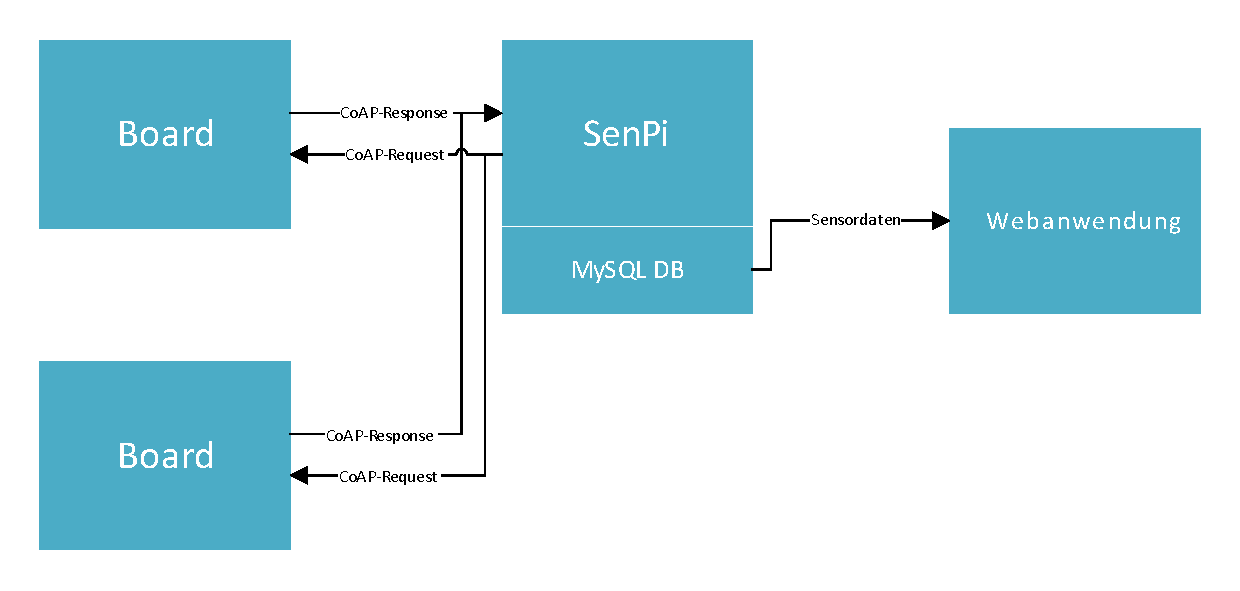
\includegraphics[scale=0.7]{interactionDiagram.pdf}
\caption{\label{fig:interacion}Interaktionen der Anwendungskomponenten}
\end{figure}


Der genaue Ablauf der Anfragen an die Boards, ist in Abbildung \ref{fig:seq_diagram} 
dargestellt.
\begin{figure}[h]
\centering
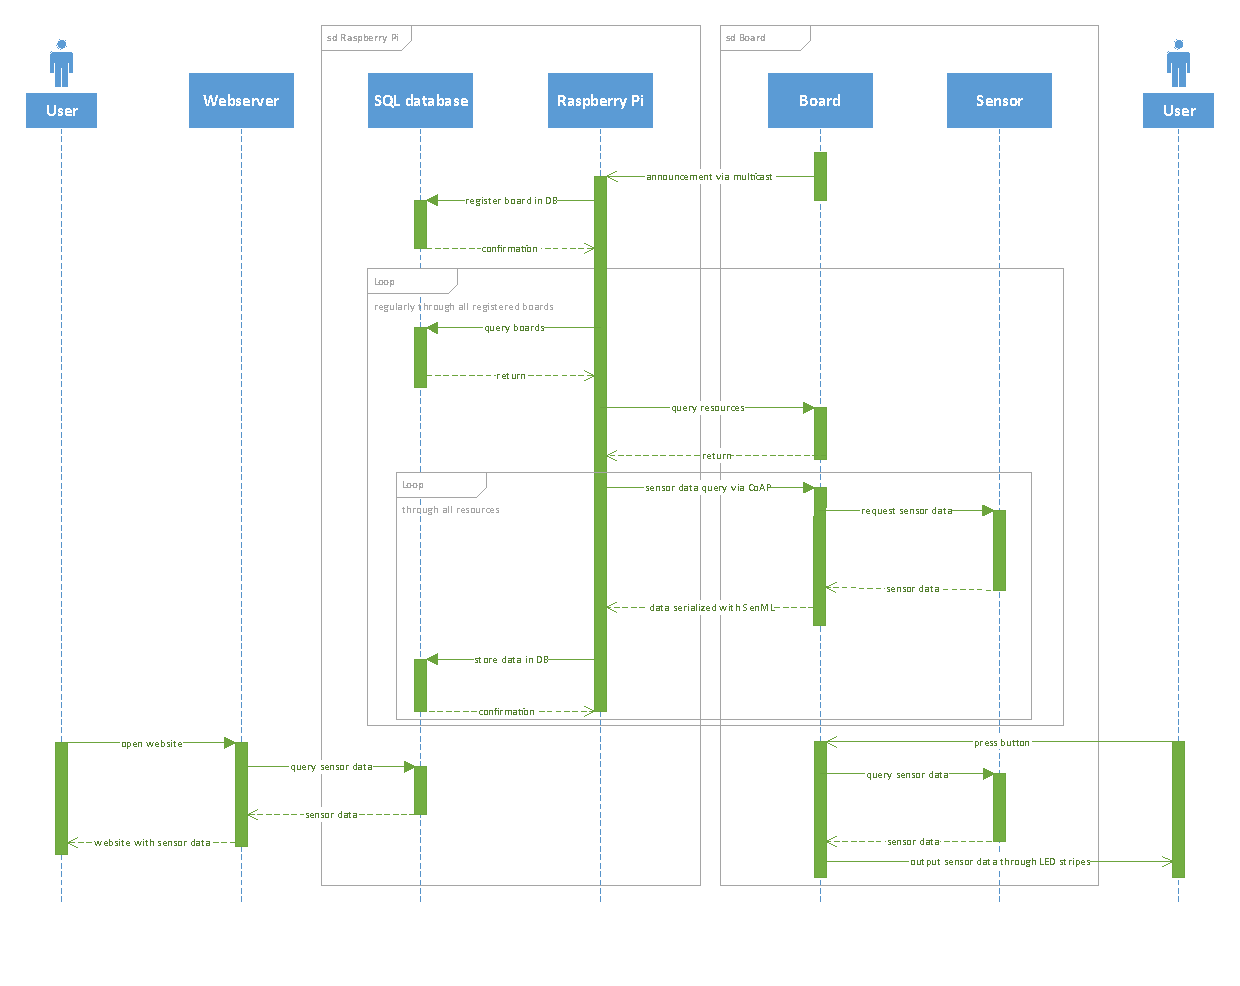
\includegraphics[scale=0.5]{sequenceDiagram.pdf}
\caption{\label{fig:seq_diagram}Sequenzdiagramm der Anwendung}
\end{figure}

\end{document}